\chapter{Technological Alternatives}
\section{Power Line Communication (PLC)}

Power Line Communication (PLC) is a technology for data communication on a conductor used also for carrying electric power. PLC systems operate by impressing a modulated carrier signal on the power wiring system. The frequency bands used by the PLC systems depends on the power wiring used and the signal transmission characteristics. The metered data can be collected at the consumer's premises and this data can be transmitted over the power lines to the supplier.

PLC systems provides variable data rates depending on the frequency of the carrier signals used. Single carrier Narrow-Band (NB) provides data rates of few kbps with carrier wave frequency varying from 20 to 200 kHz. On the other hand, Broad-Band systems (BB), operating at higher frequencies (2-30 MHz),  provide data rates of upto 200 Mbps \cite{PLC_galli}. NB-PLC and BB-PLC provide a platform for bi-directional communication and are capable of handling real-time data thus enabling utilities to identify and even predict equipment failures. There is considerable evidence that PLCs can provide point-to-point configurations on the Medium Voltage (MV) segment of the distribution grid and point-to-multipoint configurations on the Low Voltage (LV) segment of the distribution grid \cite{PLC_galli}. 

The significant advantage of PLC systems is that the deployment costs are comparable to the wireless alternatives as no additional infrastructure is required for communication and the power lines can be used for both power transmission and the communication of metered data.

\fxnote*{Verify the fact}{Power lines were set up not for the purpose of transmission of data but for the transmission of power, the power wire circuits have limited ability to carry higher frequency signals. The power line channel is frequency selective, time-varying and noisy, this implies the channel is difficult to model.} Although PLC based Advanced Metering Infrastructure (AMI) has a proven track record, it lacks  \fxnote*{highlight y this is need generally and in particular to Germany}{standardization} and this could be a major factor with respect to the large scale commercial adaptation of PLC systems for AMI \cite{PLC_galli}. Apart from the technical aspects of PLC systems, there are various governmental regulations and business requirements that dictate the mass acceptance of the technology. For example, the EU regulations does not allow for the use of BB-PLC due to stricter limitations on the allowable transmit power. 

\subsection{IPv6 and PLC}

An alternative idea is to use the IEEE 802.15.4 standard \cite{IEEE_802.15} for the physical and media sub-layers to transport IPv6 packets. Although the IEEE 802.15.4 standard is for a wireless medium at the physical layer, successful adaptation of the standard to the power line medium at the physical layer was presented in \cite{IP_PLC}. IPv6 extends the IP address space from 32 to 128 bits and solves some very important issues, such as auto configuration, security, and multicasting. This is increasingly necessary in the growing ``Internet of things".

The proof-of-concept implementation of IPv6 over PLC \cite{IP_PLC}, uses PLC nodes that are architecturally similar to classic RF based IEEE 802.15.4 nodes. These nodes are powered by micro-controllers and the communication is handled by a PLC transceiver which emulates a radio transceiver. The micro-controller deals with the IEEE 802.15.4 data format and the upper layers of the communication stack while the transceiver provides a modem with a throughput of 10 kbps. However, there are some adaptations within the MAC part of the protocol. These adjustments provide a communication over a power line using the 802.15.4 frame format. 

\section{IPv6 over Low power Wireless Personal Area Networks (6LoWPAN)}

Low-power and Lossy Networks (LLNs) refer to networks that are composed of highly constrained nodes (limited power, memory, and CPU) connected by ``lossy" links (low power radio links or PLC). A LoWPAN is a particular type of LLN, formed by devices/nodes complying with the IEEE 802.15.4 standard. The 6LoWPAN standard provides for header compression and encapsulation mechanism, that allows IPv6 packets to be communicated over IEEE 802.15.4 based networks.

Typical characterisitcs of LoWPAN nodes \cite{6LPN_dna_draft,6LPN_prob_rfc}:
\begin{itemize}
\item Short range: The operating range of the nodes is about 10 meters.
\item Low power: The transmission power of the nodes is set at around 0 to 3dBm.
\item Low memory: The nodes have typically around \fxnote*{lots of mem - but it is from RFC}{512 KB} of Flash memory.
\item Limited processing power: Although certain devices exist with 16-bit and 32-bit cores, the smallest common nodes have 8-bit processors with clock rates around 10 MHz.
\item Low bit rate: A maximum over-the-air data rate of 250 kbps is achieved by most types of the nodes.
\end{itemize}

\fxnote{Describe the pros and cons of 6LoWPAN here}

\section {Host Identity Protocol (HIP)}

\fxnote{Entire section has to be modified and shortened, probably not going with HIP}
IP address and DNS names constitute the two important global namespaces. Semantic overloading and functionality extensions have complicated these namespaces and as a result introduced a number of weaknesses. There are three critical deficiencies with the current namespaces.  First, anonymity is not provided in a consistent, trust-able manner. Second, dynamic readdressing cannot be directly managed and finally, authentication for systems and datagrams is not provided.

\begin{figure}[htb!]
\centering
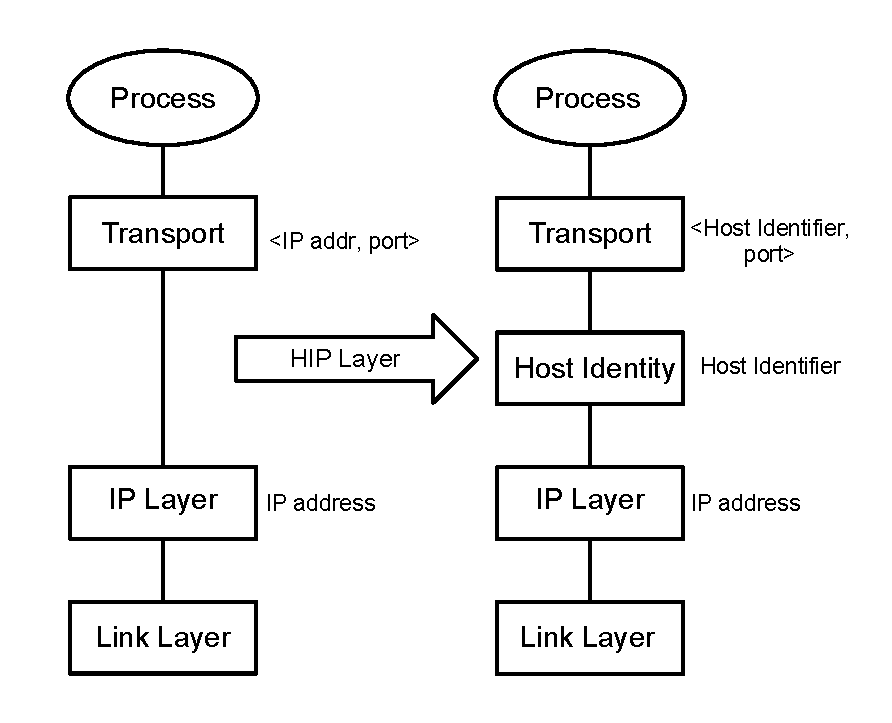
\includegraphics[width=0.8\textwidth]{images/HIP_figure1}
\caption{HIP architecture}
\label{fig:HIP_arch}
\end{figure}

HIP \cite{HIP_rfc} proposes a new namespace consisting of Host Identities and Host Identifiers (HI). There is a subtle but important difference between the two. Host Identifier is cryptographic in nature; it is the public key of an asymmetric key-pair where as a Host Identity refers to an abstract concept assigned to a `computing platform'. Each host is uniquely identified by a Host Identity and a corresponding Host Identifier (see Figure~\ref{fig:HIP_arch}). Note that however a single host can have more than one Host Identity.

In the current IP architecutre, IP addresses act as both locators and end point identifiers. That is, the IP addresses act as a routing direction vector that identifies  topological location in the Internet besides naming the physical network interface at the point-of-attachment. With HIP, the end-point names and locaters are two distinct entities. IP addresses continue to act as locators, while the Host Identifiers correspond to end-point names as shown in Figure~\ref{fig:HIP_arch}. 

With the use of HIP, transport layer protocols are no longer bound to a single IP address but to Host Identities. This enables HIP to provide for process migration and clustered servers.

The main objectives of HIP are to enhance mobility, provide for limited forms of trust between systems, dynamic IP renumbering and multi-homing. The Host Identifiers can be used in many authentication systems, such as the Internet Key Exchange (IKEv2) protocol, thus the payload traffic between HIP host is typically, but not necessarily protected with IPsec and in turn makes these payload IP packets no different from the standard IPsec protected IP packets. In other words, HIP can be seen as a special case of using IPsec thus building on top of the existing IPsec infrastructure.

\subsection{Host Identity Namespace}

A Host Identifier is a name in the Host Identity namespace, Host Identifiers represents a statistically globally unique name for naming any system with an IP stack. Although, any name that claims to be ‘statistically globally unique’ may serve as a Host Identifier, a public key of a public key pair is best recommended for an Host Identifier \cite{HIP_rfc}. 

HIP provides optional cryptographic features, however the protocol with its cryptographic features provides the complete set of functionality as advertised by the RFC. Hence using the public key as the Host Identifier avoids the need for an additional name. The Host Identifiers can be public or private i.e., they can be published or unpublished. The public Host Identifiers are stored in DNS or LDAP directories. Alternatively these identifiers can also be stored in various kinds of Public Key Infrastructure (PKI) and hence extending the scope of a Host Identifier beyond the purpose of host identification.

\subsection{The Protocol Overview}
Normal operation of HIP uses a Host Identity Tag. A HIT is a 128 bit representation of a Host Identity and is a cryptographic hash of the corresponding Host Identifier. The purpose of HIT is to enable a consistent representation of the Host Identity irrespective of the cryptographic algorithms used and to provide easier protocol encoding because of its fixed length. As HIT is used to identify the sender and recipient of a packet, it should be unique in the whole IP universe and in the case of a collision the Host Identifiers (public keys) will make the final difference.

\begin{figure}[htb!]
\centering
\includegraphics[width=0.8\textwidth]{images/HIP_figure2}
\caption{HIP base exchange}
\label{fig:HIP_be}
\end{figure}

The actual Host Identity Protocol (HIP) is composed of two two-round-trip, end-to-end Diffie-Hellman key exchange protocol, a mobility exchange and some additional messages. The purpose of the HIP base exchange (see Figure~\ref{fig:HIP_be}) is to create assurance that the peers indeed possess private keys corresponding to their host identifiers (public keys). In consequence, the base exchange creates a pair of IPsec Encapsulated Security Payload (ESP) Security Associations (SAs), one in each direction.

\begin{figure}[htb!]
\centering
\includegraphics[width=0.8\textwidth]{images/HIP_figure3}
\caption{HIP with DNS}
\label{fig:HIP_DNS}
\end{figure}

Figure~\ref{fig:HIP_be} shows the process of base exchange. First the initiator looks up Host Identifier/HIT of the responder from DNS or RVS (Rendezvous Server). Figure~\ref{fig:HIP_DNS} depicts the procedure for HIP with DNS. On the client side, the application sends DNS query to a DNS server. The DNS server replies with the Host Identifier (FQDN-\textgreater HI) instead of IP address. In a second step, another lookup is made in the Host Identity layer by the HIP daemon. This time, Host Identities are translated into IP addresses (HI-\textgreater IP) for network layer delivery.

The transport protocol sends a packet containing server's Host Identifier. The Host Identity layer replaces the Host Identifier with corresponding IP address of the server. The network layer transmits this packet with an IP header. Accordingly, the 5-tuple socket becomes \{protocol, source HI, source port, destination HI, destination port\} from the conventional \{protocol, source IP, source port, destination IP, destination port\}. 

HIP uses a special IPsec ESP mode called Bound End-to-end Tunnel (BEET). The new mode provides limited tunnel mode semantics without the regular tunnel mode overhead.

\subsection{Mobility}
\begin{figure}[htb!]
\centering
\includegraphics[width=0.8\textwidth]{images/HIP_figure4}
\caption{Mobility with HIP}
\label{fig:HIP_mob}
\end{figure}

Since the SAs are not bound to IP addresses, the host is able to receive packets that are protected using a HIP-created ESP SA from any address. Thus, a host can change its IP address and continue to send packets to its peers. Figure~\ref{fig:HIP_mob} depicts the mobility process. In the beginning, the mobile host is at address 1 and it moves to the address 2 later. During the mobility process, the mobile host is disconnected from the peer host for a brief period of time while it switches from address 1 to address 2. Upon obtaining a new IP address, the mobile host sends a \texttt{LOCATOR} parameter to the peer host in an \texttt{UPDATE} message. The \texttt{LOCATOR} indicates the new IP address, the IPsec - Security Parameters Index (SPI) associated with new IP address, the address lifetime and whether the new address is a preferred address. The peer host performs an address check and solicit a response from the mobile host. Depending on whether the mobile host has initiated a rekey, and on whether the peer host itself wants to rekey to verify the mobile host's new address, the process can be categorized into three cases: 
\begin{itemize}
\item Readdress without rekeying, but with an address check, as in Figure~\ref{fig:HIP_mob}; 
\item Readdress with a mobile-initiated rekey; and 
\item Readdress with a peer-initiated rekey.
\end{itemize}

\subsection{Multihoming}
\begin{figure}[htb!]
\centering
\includegraphics[width=0.8\textwidth]{images/HIP_figure5}
\caption{Multihoming with HIP}
\label{fig:HIP_mhom}
\end{figure}
A host can sometimes have more than one interface. The host may notify the peer host of the additional interfaces by using the \texttt{LOCATOR} parameter. In Figure~\ref{fig:HIP_mhom} the multihoming host is assumed to have two IP addresses, \textit{addr1} and \textit{addr2}. Further, \textit{addr1} is assumed to be the preferred address. The multihoming host sends an \texttt{UPDATE} packet including \textit{addr1} and \textit{addr2} to its peer host. The peer host sends \texttt{UPDATE} packets to each address and updates corresponding SPIs.